\chapter{Método Propuesto}

Una forma de establecer equivalencias entre un recurso FHIR y un arquetipo de integración openEHR es identificando relaciones entre elementos de datos del recurso FHIR y restricciones del arquetipo de integración openEHR. Para ello se crea un arquetipo de integración openEHR a partir de la definición del recurso FHIR existente.

La creación del arquetipo de integración openEHR a partir de la definición del recurso FHIR utilizando equivalencias entre tipos de datos puede ser sencilla. El arquetipo de integración openEHR se puede crear de forma manual dentro de un editor de arquetipos como los citados en \cite{openEHRModellingTools}. Este se modela con la misma estructura del recurso FHIR. Cada tipo de dato de FHIR de la estructura se sustituye por su equivalente tipo de dato de openEHR. En este trabajo, se presenta una alternativa diferente consistente en la creación a través de un proceso automatizado. Las ventajas de la creación automática son tiempo de creación y riesgo de introducir errores por factor humano menores a los de la creación manual.

\section{Equivalencias entre tipos de datos}

La definición de un elemento en un recurso FHIR incluye tipo de dato \cite{FHIRElement}. Por lo tanto, un prerequisito es encontrar equivalencias entre tipos de datos FHIR y tipos de datos openEHR. Las equivalencias permitirán crear arquetipos openEHR a partir de definiciones de recursos FHIR.

Dada la función \( f(x) \) que retorna el dominio de valores que se le puede asignar a un dato \( x \), \( A \) el conjunto de atributos del tipo de dato de openEHR \( o \), la equivalencia entre el tipo de dato de FHIR \( p \)  y el tipo de dato de openEHR \( o \) existe si se cumplen las condiciones de:

\begin{enumerate}
  \item \( \exists a \in A \land f(a) \supseteq f(p) \);
  \item los propósitos de \( o \) y \( p \) son similares.
\end{enumerate}

Las equivalencias se encuentran al realizar una revisión manual exhaustiva del conjunto de tipos de datos de FHIR \cite{FHIRDataTypes} y del Modelo de Información de Tipos de Datos de openEHR \cite{openEHRDataTypes}. En primer lugar, para cada tipo de dato de FHIR se agrupa los tipos de datos de openEHR que tengan algún atributo cuyo dominio de valores sea un superconjunto del dominio de valores del tipo de dato de FHIR. Posteriormente, se analiza y compara las definiciones, incluyendo el propósito, de cada tipo de dato de FHIR y su grupo de tipos de datos de openEHR encontrados inicialmente. Solo para el tipo de FHIR boolean se utiliza la definición de \cite{W3C} por no tener una definición explícita en la especificación de FHIR y por ser un tipo de dato importado desde W3C.

Como ejemplo, el tipo de FHIR boolean y el tipo de openEHR DV\_BOOLEAN reúnen ambas condiciones, por lo tanto, son equivalentes:
\begin{enumerate}
  \item los valores true y false del dominio de valores del tipo boolean pueden ser almacenados dentro del atributo value del tipo DV\_BOOLEAN;
  \item el uso de DV\_BOOLEAN, el cual especifica que el tipo se usa para elementos que son datos verdaderamente booleanos, es el mismo uso que tiene el tipo de dato boolean.
\end{enumerate}

Solo los tipos de datos primitivos de FHIR requieren una equivalencia con los tipos de datos openEHR.

\section{Proceso automatizado}

El proceso automatizado se basa en la formalización propuesta en \cite{Maldonado09}, la cual para la definición de la sección de arquetipos usa un sistema de tipos sobre una estructura de árbol. El sistema de tipos modela las restricciones estructurales impuestas por los arquetipos sobre el modelo de referencia. La base del sistema de tipos es la lista de multiplicidad restringida (CML por sus siglas en inglés). El CML es un lenguaje de definición que dentro de la definición del tipo especifica la secuencia válida de hijos de un nodo atributo o objeto de un arquetipo.

El proceso automatizado tiene 3 etapas como se muestra en la Figura \ref{fig:solution}: abstracción, sustitución y definición. Las etapas se repiten por cada arquetipo de integración openEHR a crearse a partir de cada recurso FHIR.

\begin{figure}[h]
  \centering
  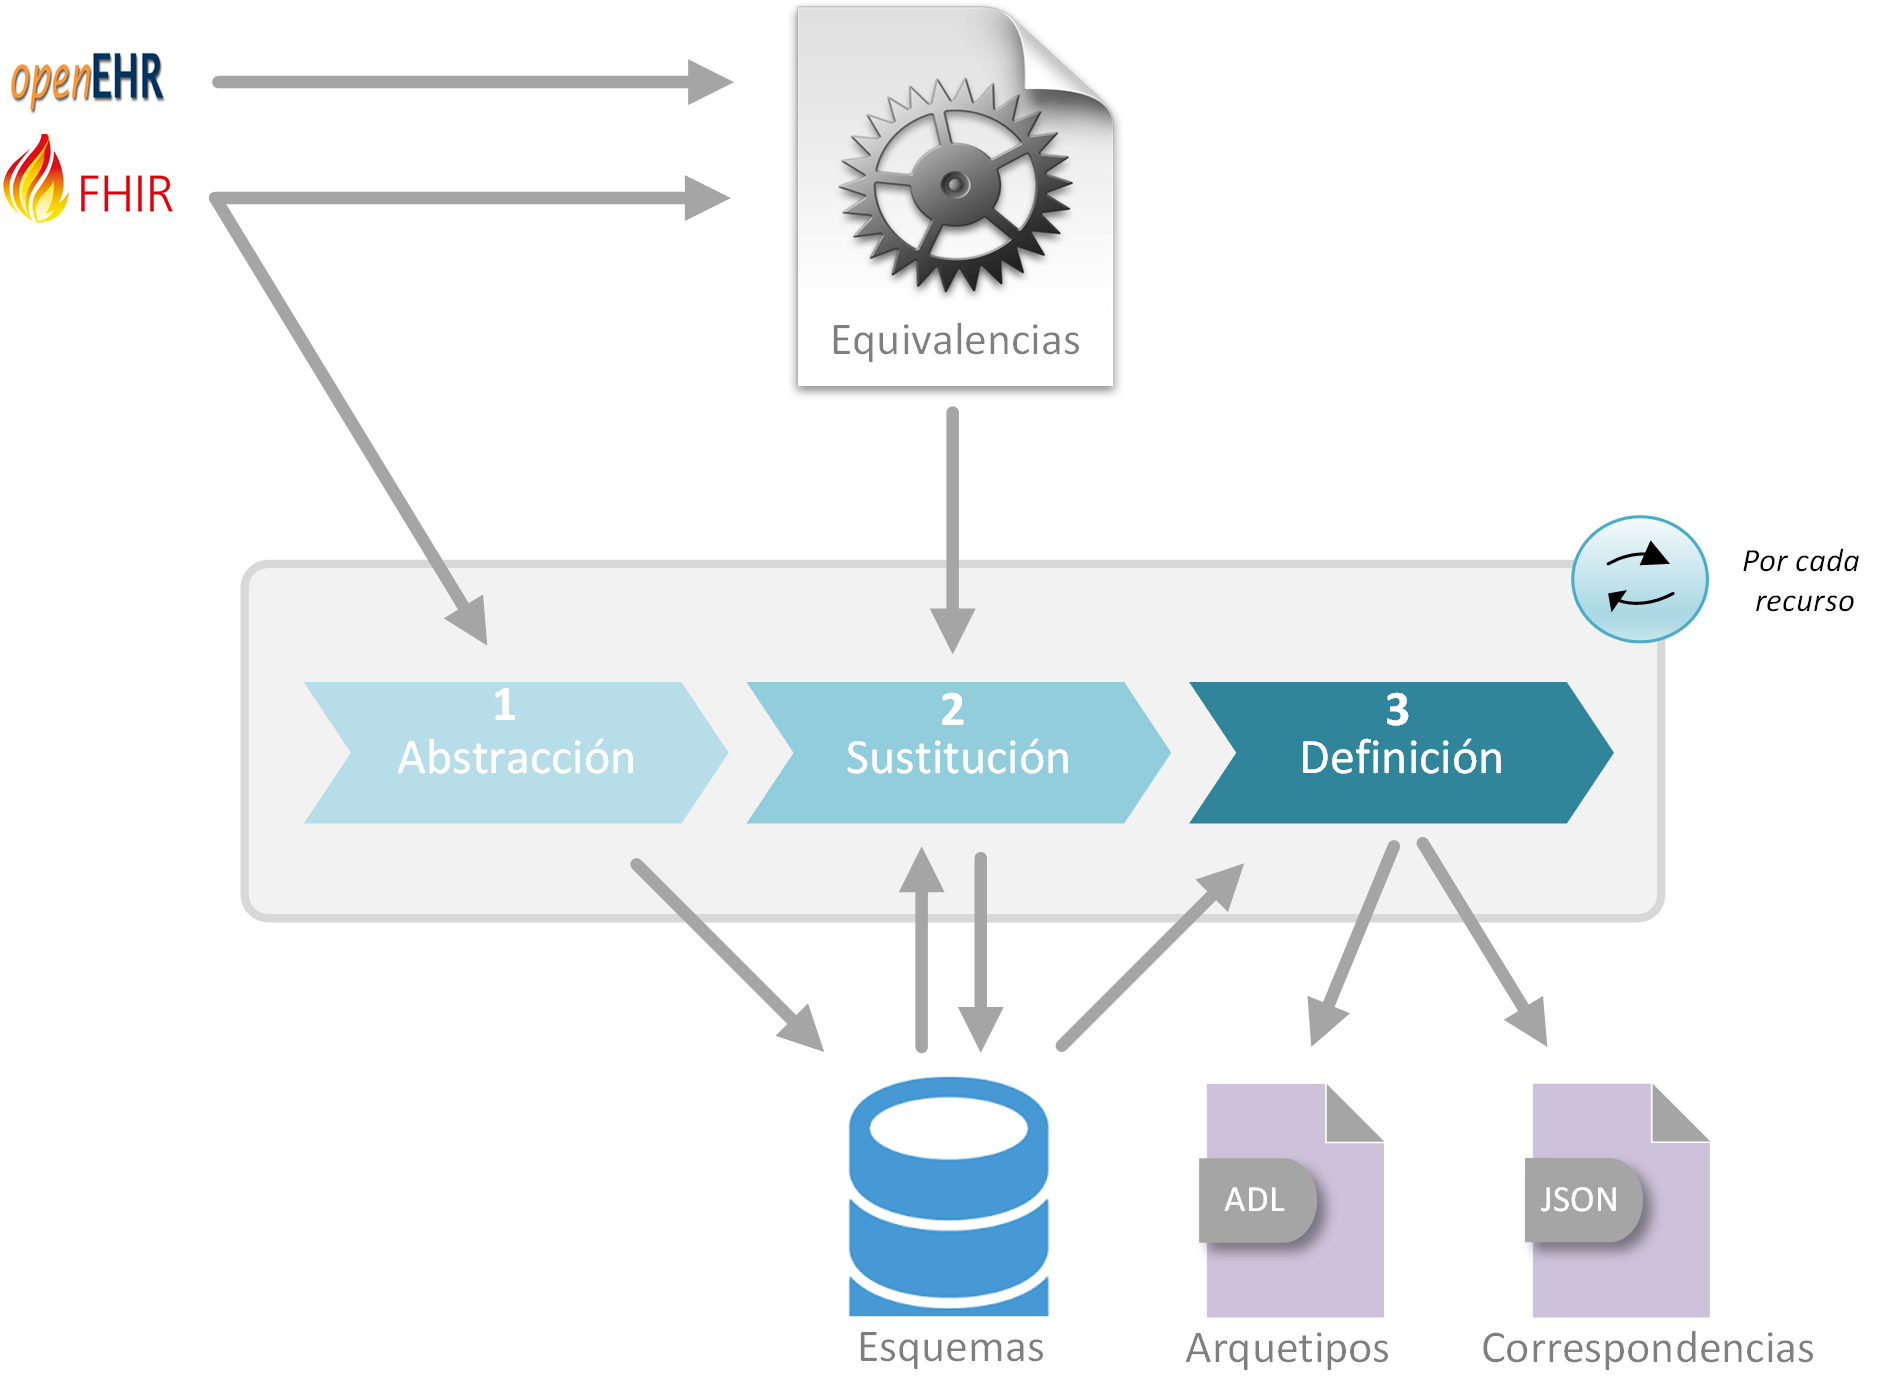
\includegraphics[scale=0.5]{./images/solution.png}
  \caption{Proceso automatizado.}
  \label{fig:solution}
\end{figure}

\subsection{Etapa de abstracción}

El recurso FHIR se modela dentro de un sistema de tipos similar al desarrollado en \cite{Maldonado09}. Cada elemento del recurso FHIR se abstrae por el tipo que describe su estructura. La definición de un tipo es de la forma:

\begin{align*}
T_t:=p_t\{h_t\}
\end{align*}

\noindent
donde \(T_t\) es el nombre del tipo \(t\), \(p_t\) es el predicado que describe los valores soportados por el tipo \(t\) y \(h_t\) es un CML que especifica los elementos hijos que puede tener el tipo \(t\).

La definición del recurso FHIR \(R\) con elementos \(E_1\), \dots , \(E_2\) se abstrae con la definición de tipo como sigue:

\begin{align*}
T_R:=es\_R\{T_{E_1}^{(min_{E_1} \colon max_{E_1})} \dots T_{E_2}^{(min_{E_2} \colon max_{E_2})}\}
\end{align*}

\noindent
donde \(T_{E_1}\) es el tipo que define el elemento \(E_1\), \(min_{E_1}\) y \(max_{E_1}\) son los límites inferior y superior respectivamente de las veces que se permite que el elemento \(E_1\) aparezca en el recurso \(R\). La diferencia con el CML introducido en \cite{Maldonado09} es que en la definición de un tipo no se utilizan las restricciones de longitud por no agregar información adicional a la abstracción de un recurso FHIR.

Para modelar vinculaciones, se extiende el sistema de tipos presentado en \cite{Maldonado09}, agregando definiciones de vinculación. Una definición de vinculación es de la forma:

\begin{align*}
[T_E] := CV
\end{align*}

\noindent
donde \(T_E\) es la definición del tipo del elemento al cual se le vincula el conjunto de valores \(CV\).

Por ejemplo, al considerar el recurso SimplePatient (simplificación del recurso FHIR Patient \cite{FHIRPatient}) que modela un paciente que tiene un solo elemento gender del tipo code \cite{FHIRDataTypes} vinculado al conjunto de valores AdministrativeGender \cite{FHIRAdministrativeGender}, se modela por el conjunto de tipos:

\begin{align*}
&T_{SimplePatient}:= \\
&\qquad es\_SimplePatient\{T_{SimplePatient.gender}^{(0:1)}\} \\
&T_{SimplePatient.gender}:= \\
&\qquad es\_gender\{T_{SimplePatient.gender.code}^{(1:1)}\} \\
&T_{SimplePatient.gender.code}:= \\
&\qquad es\_code\{\epsilon\} \\
&[T_{SimplePatient.gender.code}] := \\
&\qquad URL \footnotemark[1] \\
\end{align*}

\footnotetext[1]{https://www.hl7.org/fhir/valueset-administrative-gender.html}
Un conjunto de tipos que define un recurso FHIR se denomina esquema FHIR en este trabajo.

\subsection{Etapa de sustitución}

El esquema basado en tipos de datos FHIR generado en la etapa previa se transforma en un esquema basado en tipos de datos openEHR. Si se considera las definiciones de un tipo FHIR y de un tipo openEHR:

\begin{align*}
&T_{FHIR}:=p\_FHIR\{h_{FHIR}\} \\
&T_{OPENEHR}:=p\_OPENEHR\{h_{OPENERH}\}
\end{align*}

\noindent
Y existe una equivalencia entre ambos tipos según las condiciones mencionadas en la sección equivalencias entre tipos de datos:

\begin{align*}
&T_{FHIR} = T_{OPENEHR}
\end{align*}

\noindent
Entonces por relación transitiva:

\begin{align*}
p\_FHIR\{h_{FHIR}\} = p\_OPENEHR\{h_{OPENEHR}\}
\end{align*}

\noindent
Por tanto ambas expresiones son intercambiables entre sí y la sustitución es directa. Cada definición de un tipo de dato FHIR se reemplaza por una definición de tipo de dato openEHR equivalente. Cada definición de vinculación sobre un tipo de dato FHIR se sustituye por una definición de vinculación sobre un tipo de dato openEHR equivalente.

Por ejemplo, el esquema FHIR del recurso SimplePatient se transforma al reemplazar la definición del tipo FHIR code por la definición del tipo openEHR DV\_TEXT equivalente en:

\begin{align*}
&T_{SimplePatient}:= \\
&\qquad es\_SimplePatient\{T_{SimplePatient.gender}^{(0:1)}\} \\
&T_{SimplePatient.gender}:= \\
&\qquad es\_gender\{T_{SimplePatient.gender.DV\_TEXT}^{(1:1)}\} \\
&T_{SimplePatient.gender.DV\_TEXT}:= \\
&\qquad es\_DV\_TEXT\{T_{SimplePatient.gender.DV\_TEXT.value}^{(1:1)}\} \\
&T_{SimplePatient.gender.DV\_TEXT.value}:= \\
&\qquad es\_value\{T_{string}^{(1:1)}\} \\
&[T_{SimplePatient.gender.DV\_TEXT.value}] := \\
&\qquad URL \footnotemark[1] \\
&T_{string}:= \\
&\qquad es\_string\{\epsilon\} \\
\end{align*}

Un esquema basado en tipos de datos openEHR se le denomina esquema openEHR en este trabajo. Como se observa, los esquemas FHIR y openEHR de SimplePatient conservan la misma estructura que la definida por el recurso SimplePatient.

\subsection{Etapa de definición}

Según las definiciones de un esquema openEHR, se crea un arquetipo de integración openEHR usando Archetype Definition Language (ADL) \cite{openEHRADL}.

Como identificador del nuevo arquetipo openEHR se usa un nombre de espacio fhir y el nombre del recurso FHIR que el esquema openEHR modela. Por ejemplo, el identificador del arquetipo openEHR del recurso SimplePatient es:

\begin{lstlisting}
fhir::openEHR-EHR-CLUSTER.SimplePatient.v1.0.0
\end{lstlisting}

Para la definición del nuevo arquetipo openEHR, los tipos del esquema openEHR abstraídos de tipos primitivos de FHIR son expresados usando la estructura ELEMENT, y los demás tipos del esquema openEHR son expresados usando la estructura CLUSTER. Ambas estructuras pertenecen al Modelo de Información de Estructuras de Datos de openEHR \cite{openEHRDataStructures}. Por ejemplo, la sección de definición del arquetipo openEHR del recurso SimplePatient usa las clases openEHR CLUSTER y openEHR ELEMENT para los tipos \(T_{SimplePatient}\) y \(T_{SimplePatient.gender}\) respectivamente:

\begin{lstlisting}[mathescape=true]
CLUSTER[id1] $\in$ {
  items $\in$ {
    ELEMENT[id2] occurrences $\in$ {0..1} $\in$ {
      value $\in$ {
        DV_TEXT[id3]
      }
    }
  }
}
\end{lstlisting}

Las definiciones de vinculación se agrega en la sección de vinculación de términos del nuevo arquetipo openEHR. Por ejemplo, la definición de vinculación del tipo \(T_{SimplePatient.gender.DV\_TEXT.value}\) del recurso SimplePatient se transcribe en la sección de vinculación de términos de su arquetipo openEHR equivalente:

\begin{lstlisting}[escapechar=$]
term_bindings = <
  [``fhir"] = <
    [``id3"] = < URL$\footnotemark$ >
  >
>
\end{lstlisting}

\footnotetext{https://www.hl7.org/fhir/valueset-administrative-gender.html}

Los arquetipos openEHR permiten las formaciones de rutas ADL, las cuales sirven para identificar elementos de los arquetipos openEHR \cite{openEHRArchitecture}. En esta etapa, se crea las rutas ADL del nuevo arquetipo openEHR y se relaciona con las rutas de los elementos de su recurso FHIR equivalente. Considerando el recuso de SimplePatient, la relación que se establece es:

\begin{lstlisting}[mathescape=true]
SimplePatient.gender $\Leftrightarrow$ /items[id2]/value[id3]
\end{lstlisting}
